\begin{figure}[tbp]
\centering
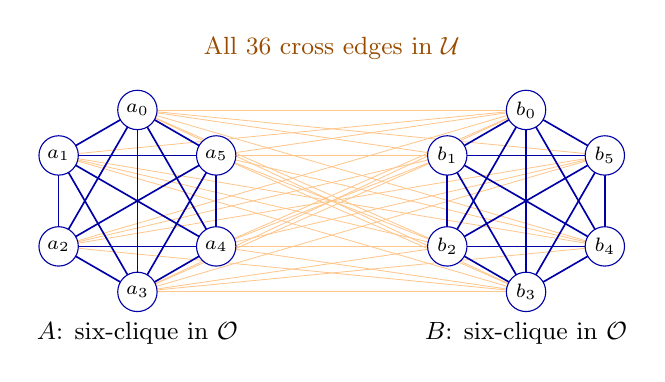
\begin{tikzpicture}[scale=1.05,
 dot/.style={circle,draw=blue!65!black,fill=white,inner sep=0pt,
 minimum size=5mm,font=\scriptsize}]
\foreach \i in {0,...,5} {
 \coordinate (a\i) at ({-2.35+1.1*cos(90+60*\i)},{1.1*sin(90+60*\i)});
 \coordinate (b\i) at ({2.35+1.1*cos(90+60*\i)},{1.1*sin(90+60*\i)});
}
\foreach \i in {0,...,5} \foreach \j in {0,...,5}
 \draw[orange!45,line width=.3pt] (a\i)--(b\j);
\foreach \i in {0,...,5} \foreach \j in {0,...,5} {
 \ifnum\i<\j
  \draw[blue!65!black,line width=.6pt] (a\i)--(a\j);
  \draw[blue!65!black,line width=.6pt] (b\i)--(b\j);
 \fi
}
\foreach \i in {0,...,5} {
 \node[dot] at (a\i) {$a_{\i}$};
 \node[dot] at (b\i) {$b_{\i}$};
}
\node[font=\small] at (-2.35,-1.6) {$A$: six-clique in $\mathcal O$};
\node[font=\small] at (2.35,-1.6) {$B$: six-clique in $\mathcal O$};
\node[font=\small,text=orange!60!black] at (0,1.85) {All $36$ cross edges in $\mathcal U$};
\end{tikzpicture}
\caption{Two further mutually unbiased bases would require twelve
distinct vector-ball labels: six pairwise orthogonality-compatible labels
in each set, with every cross pair unbiasedness-compatible. The graphs
retain all necessary edges. A completed search excluding this pattern
therefore excludes the two bases throughout the phase ball.}
\label{fig:two-cliques}
\end{figure}
